StreamStory is a client-server application, with its front-end implemented in HTML5,
CSS3 and JavaScript. The page layout is handled by Twitter Bootstrap 3, providing 
responsiveness and scalability \lstopar{to} all types of devices. We use Cytoscape.js
for visualization of graphs and trees, while D3.js is user for visualization of charts.
The front-end relies on technologies line Ajax and WebSockets for real-time transparent
updates.

The backend uses a hybrid implementation with its core functionality written in C++
as part of the QMiner \cite{qminer} data analytics platform, under the BSD license
and exposed as a Node.js addon running on Googles V8 JavaScript environment. Node.js
thus acts as glue and exposes the functionality through RESTful web services
using Express, also taking care of session management. Login information is stored
in a MySQL database.

Having the core functionality implemented in C++ provides performance benefits, especially
when dealing with larger datasets. When using StreamStory, the most time consuming \lstopar{part}
is the initial model construction. Indeed, after the initial step, everything is real-time.
The model construction process includes clustering the dataset, aggregating states,
computation of state statistics, state assistance services and laying out the generates
hierarchical graph on a plane with the most time consuming tasks being modeling the state
transitions and the computation of state assistance, as the system trains logistic regression
and decision tree models for each state in the hierarchy. These tasks are however independent
for each state and can be parallelized. To measure the performance, we constructed models on two datasets
of sizes 155MB (285k instances) and 500MB (\lstopar{3M} instances) respectively. A preselected
set of five attributes was randomly chosen for each dataset and used in all the experiments. We
then constructed models with 18, 38 and 78 states respectively. Figure \ref{fig:performance} shows
\lstopar{a graph of constructions times}.
\begin{figure}[h!]
	\centering
	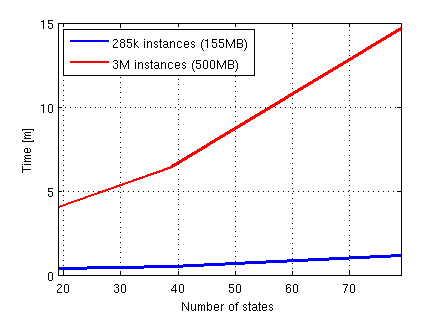
\includegraphics[width=0.7\columnwidth]{time-measurements}
	\caption{\lstopar{[TODO]}.}
	\label{fig:performance}
\end{figure}

\iffalse
\begin{tabular}{ c | c c c c c}
	\label{tab:time-tests}
	 & 10 & 20 & 40 & reading CSV & file size \\
	\hline
	3229541 & 11min & 13min 32s & 21min 50s & 6:58,7:05,7:10 & 500MB \\
	285168 & 1:31 & 1:36 & 2:17 & 1:09,1:06,1:08 & 155MB
\end{tabular}
\fi